\chapter{Methods}\label{ch: methods}

This chapter describes the methods for the simulation study. This study is intended to validate the power approximation introduced in the last chapter for the cluster-robust Wald test of a study-level moderator with multiple categories (Equation \ref{eq: multiple_categories_satt}). To answer my three research aims (Section \ref{sec: aims}), I estimated two types of power: estimates of true power of the HTZ test based on the CHE+RVE model through a Monte Carlo simulation and estimates of power from the approximation formula. For each simulation design condition, I compared the estimates of power resulting from the approximation with the average of all simulated rejection rates for the Wald test of multiple categories estimated using a CHE+RVE model. I obtained the two types of power estimates independently, and then I examined the discrepancies between them when addressing my first and second aims. For the third aim, I assessed the performance of the cluster-robust Wald test for multiple categories of a study-level categorical moderator by evaluating empirical Type I error rates using only the true power estimates. 
%To validate the approximation, I estimate the true power levels of HTZ test based on the CHE+RVE model through a Monte Carlo simulation. 
In the following sections, I provide an overview of the process of simulating meta-analytic datasets and the estimation methods applied to each dataset. Then, I detail how I estimated the power from the approximation formula and operationalized assumptions about the distribution of sampling variances and the number of effect sizes per study. Then, I outline the experimental design and the performance criteria.    

%Additionally, for the approximations, I will evaluate three different ways to assume the study characteristics of the number of effect sizes per study and sample variance of the effect sizes (three ways from \textcite{vembye2023} and one additional way): 1) empirical distributions of the data-generating dataset  2) stylized distributional assumptions 3) assuming perfect balance across studies.

\section{Methods for the Simulation to Estimate True Power}

In the sections below, I first detail how I generated the meta-analytic datasets and the estimation methods used to estimate the true power of the CHE+RVE model. 

%This simulation was run separately from the approximation study, but both used the same design conditions (more details in Section \ref{sec:simulationdesgin}) and the same empirical dataset for sampling the within-study characteristics. 

\subsection{Data Generation for the Monte Carlo Simulated Data}

I generated simulated data through a series of steps following the procedures used in \textcite{vembye2023} and \textcite{pustejovsky2022} to generate the SMD effect sizes. However, I deviated from those methods when generating the design matrix and the vector of meta-regression coefficients. The following condition parameters were specified to generate a simulated dataset: the number of categories of the categorical moderator, $C$; total number of studies in the dataset, $J$; the balance of the number of studies per category across the moderator, balanced $j_c$ or imbalanced $j_c$; the pattern of the regression coefficients from a no-intercept model, or in this context, the pattern of the overall pooled effects of each category, $f_c$; the number of effect sizes per study, $k_j$; the sampling variances, $\sigma_j^2$; the between-study heterogeneity, $\tau$; the within-study heterogeneity, $\omega$; the sampling correlation, $\rho$; and the ``power neighborhood'' used to obtain the true power estimates and the approximated power, $P$. 

Using the specified parameters above, the simulated meta-analytic data were generated in four steps. First, I generated the $\mu_c$ vector of regression coefficients. Second, I sampled within-study characteristics, $k_j$ and $\sigma_j^2$, from an empirical dataset. Third, I created a design matrix, $\bm{X}$. Fourth, I simulated the standardized mean difference estimates based on the correlated-and-hierarchical effects structure (CHE) model. The first three steps generated the study-level categorical moderators, and the fourth step generated the standardized mean difference estimates. In the following sections, I will be going into these steps in more detail.

\subsubsection{Generating the Design Matrix, $\bm{X}$, and the Vector of Meta-regression Coefficients, $\mu_c$} \label{sec:XandBeta}

To evaluate the approximation across a spectrum of power values, I specified a power level, referred to as the ``power neighborhood", and then I found the $\bm{\beta}$ vector of $\mu_c$ values that would result from combinations of the power neighborhood factor and the other simulation design factors. By doing this, the resulting power would be somewhat near the specified power neighborhood level. If I had instead specified the meta-regression coefficient parameters, I would have been able to evaluate only a restricted range of power levels.

The following is a high-level overview of how study-level categorical moderator values were generated. First, using the mean of effect sizes per study from an empirical distribution, the mean of the sampling variances from an empirical distribution, the between-study heterogeneity, the within-study heterogeneity, and the sampling correlation, I generated the study-level weights, $\tilde{w}_{jc}$ (Equation \ref{eq: CHEweights-study_cat}). Next, using the study-level weights and the number of categories, I calculated the degrees of freedom using Equation \ref{eq: multiple_categories_satt}. Then, given the specified power neighborhood, the generated weights, the degrees of freedom, the number of categories, and an $\alpha$-level of $.05$, I derived the non-centrality parameter of the non-central F-distribution, $\lambda$, using numerical methods. Then, given the pattern of the true effects for each category of a moderator, the study-level weights, and the generated non-centrality parameter, I found the scaling factor of the overall pooled effect for each category, $\zeta$, which is a parameter I created to be able to generate the $\mu_c$ values. Using the generated scaling factor, the pattern of the overall pooled effects, and the specified number of categories, I created the $\bm{\beta}$ vector of $\mu_c$ values. Finally, using the specified values for the number of categories, the total number of studies, and the balance of the number of studies per category across the moderator, I generated a design matrix, $\bm{X}$.

\subsubsection{Sampling Study Characteristics from Empirical Dataset}

Following the methods of \textcite{vembye2023}, for each study included in the simulated meta-analytic dataset, I sampled the number of effect sizes, $k_j$, and the sampling variances, $\sigma_j^2$, from an empirical dataset. Furthermore, I sampled the number of effect sizes and the sampling variances as pairs, because there is a possible empirical relationship between the two parameters. For the empirical dataset, I selected data from a meta-analysis conducted by \textcite{WilliamsRyan2022HiMI}, which synthesized results from 191 randomized control trials of mathematics interventions designed for school-aged children from 1991 to 2017. This study applied broad inclusion criteria and as a result captured 1,109 effect size estimates, 510 samples, and 191 studies representative of the type of data in educational research, including studies where student data is clustered at the classroom, school, and/or district level. I aimed to evaluate a large range of possible values for the number of included effect size estimates and paired sampling variances. 

Because the studies included in this meta-analysis were randomized control trials, \textcite{WilliamsRyan2022HiMI} adjusted sample variances for clustering at the level of random assignment \autocite{hedgesEffectSizesClusterRandomized2007, hedges2013}. Following the methods of \textcite{vembye2023}, I found the effective sample size by: $ESS_{ij} = \frac{4}{ \sigma_{ij}^2 }$, where $\sigma_{ij}^2 $ is the sampling variance at the effect size level.  I then averaged the effective sample size up to the study level ($ESS_j$). Finally, for standardized mean differences comparing two groups there is a relationship between the sampling variance and the sample size assuming the group sizes $\sigma^2 \approx \left( \frac{4}{ESS} + \frac{\mu^2}{2(ESS -2)} \right)$\autocite{valentine2010}. Again following the methods of \textcite{vembye2023}, I generated the average study-level sampling variance as $\sigma_j^2 = \frac{4}{ESS_j}$. After evaluating the broad range of effective sample sizes (3, 3604), I decided to subset the data to remove extremely large studies where the $ESS_j >= 500$ or $k_j >= 20$. Furthermore, the degrees of freedom of the Wishart distribution, $ESS_j-2$, needs to be greater than the number of effect sizes, $k_j$, to create a covariance matrix for the SMD effect sizes. Therefore, I removed any studies that had $k_j \leq ESS_j - 2$. The final dataset consisted of the following range of the effective sample size values: (15 , 489). After making these adjustments, the final empirical dataset is comprised of 167 study-level sampling variances, and  167 values for the number of effects per study. The arithmetic mean of the number of effects is 4.56, the harmonic mean is 2.53, and the range is (1, 18). The arithmetic mean of the sampling variances is 0.067, the harmonic mean is 0.031, and the range is (0.008, 0.267). 

%The blue lines in Figures \ref{fig:densitysigma_sq} and \ref{fig:pmfkj} show the distribution of $\sigma_j^2$ values and the empirical PMF plot of the $k_j$ values in the dataset, respectively. 

\subsubsection{Details on the Design Matrix, $\bm{X}$}
I generated the design matrix based on: factor values for the number of categories of the categorical moderator, $C$, the total number of primary studies, $J$, and the condition-specific degree of balance in the number of studies per category across the moderator, balanced $j_c$ or imbalanced $j_c$. I parameterized the meta-regression model as a no-intercept model, so the $\bm{X}$ did not include a vector of $1$'s for the first column. The $\bm{X}$ had $K \times C$ dimensions, and the form is $\bm{X} = (\bm{X}_1', \cdots, \bm{X}_J')'$ where $\bm{X}_j$ is a $k_j \times C$ matrix of covariates for study $j$. I used dummy-coded indicators for each category at the study level, so if a study fell under that category, it had a code of ``1" and a code of ``0" otherwise. 

For example, the following is the design matrix for a study-level moderator with three categories and four studies, where the first study has three effect sizes, the second study has two effect sizes, the third study has one effect size, and the fourth study has two effect sizes (using the same notation as Equation \ref{eq: no-intercept dependent}): 
\begin{equation}
  \mathbf{X} =\begin{bmatrix}
    b_{111} & b_{112} & b_{113} \\
    b_{211} & b_{212} & b_{213} \\
    b_{311} & b_{312} & b_{313} \\
    b_{121} & b_{122} & b_{123} \\
    b_{221} & b_{222} & b_{223} \\
    b_{131} & b_{132} & b_{133} \\
    b_{141} & b_{142} & b_{143} \\
    b_{241} & b_{242} & b_{243} 
   \end{bmatrix} = 
   \begin{bmatrix}
    1 & 0  & 0 \\
    1 & 0  & 0 \\
    1 & 0  & 0 \\
    0 & 0  & 1 \\
    0 & 0  & 1 \\
    0 & 1  & 0 \\
    1 & 0  & 0 \\
    1 & 0  & 0 
   \end{bmatrix} 
   \nonumber
\end{equation}
This study would be considered imbalanced since two of the studies fall under the first category, while only one study each falls under the second and third categories. 

\paragraph{Balance of the Number of Studies Across Categories} \label{sec: detailsbal}

%Because in applied meta-analyses, the total number of studies, $J$, varies in real meta-analytic datasets, it may be important to investigate how the balance of the number of studies per category impacts power. 

I evaluated two conditions for balance of the number of studies across categories, denoted as balanced $j_c$ vs. imbalanced $j_c$. The first condition, the balanced $j_c$ condition, I imposed balance across all the categories, where the same number of studies qualified for each category. In the second condition, the imbalanced $j_c$ condition, I assessed more extreme imbalances in the number of studies per category. I introduced imbalance by assigning an unequal number of studies per category, through each category having a set proportion of the total number of studies in the dataset. In the imbalanced condition, if $C = 2$, then first category with the smaller $\mu_c$ value had $\frac{1}{4} \times J$, and the other category  with the larger $\mu_c$ value had $\frac{3}{4} \times J$. If $C = 3$, then first two categories with the smaller $\mu_c$ values had $\frac{1}{4} \times J$, and the other category with the largest $\mu_c$ value had $\frac{1}{3} \times J$. Finally, if $C = 4$, then first three categories with the smaller $\mu_c$ values had $\frac{1}{6} \times J$, and the other category with the largest $\mu_c$ value had $\frac{1}{2} \times J$. I chose these proportions because all of the factors for $J$ are multiples of 12, and I wanted each $j_c$ to be an integer. 

\subsubsection{Details on the $\bm{\beta}$ Vector of $\mu_c$ Values}

To generate the vector of meta-regression coefficients, $\bm{\beta}$, I parameterized the regression model as a no-intercept model. The $\bm{\beta}$ becomes a vector of the average effect size for each category of the categorical moderator, $\mu_c$, for $c = 1, \cdots, C$. To be able to generate the $\mu_c$ values, I defined them as $\mu_c = f_c \times \zeta$,  where $f_c$ is the pattern of the $\mu_c$, and $\zeta$ is the scale of the $\mu_c$. I specified the $f_c$ as a design condition and generated the $\zeta$ from various design conditions. Below are the details on these new parameters, along with an explanation of how I generated the $\bm{\beta}$ vector.

%\subparagraph{Factors Related to Alternative Hypotheses}
\paragraph{The Patterns of the Meta-Regression Coefficients, $f_c$} \label{sec: patterns}

To determine which scenarios for the patterns of the meta-regression coefficients to include in this analysis, I specified potential alternative hypotheses applying a scenario in which not all of the $\mu_c$ are equal. There are infinite possible alternative hypotheses. The number of categories ($C$), the balance of the number of effect sizes and number of studies per category, the average effect in each category, and the spread of the overall pooled effects for each category are all factors that would impact power. The following is how I defined potential scenarios for when the magnitude of the differences between these overall pooled effects per category would impact the power.  
To examine how the alternative hypothesis specification affects power, it is necessary to define different scenarios for the average effect size per category, $\mu_c$. 
%In Table \ref{tab:patterns} below, I defined a set of patterns, $f_c$, for the values of the $\mu_c$. 
As can be seen in Table \ref{tab:patterns}, across all the patterns, $\mu_c$ is operationalized by $f_c \times \zeta$ where $\zeta$ is the scaling factor, and $f_c$ is the additive distance or pattern. These patterns are not exhaustive but are diverse in terms of the possible variations found in a given meta-analytic dataset. I am interested in how the spread and balance of the overall true effect size for each category across a variable affect power. 
%For the Additive Distance or AD pattern type, 
%For the first pattern, each $\mu_c$ is different and spaced by a value of $\zeta$. For example, the $\mu_c = [0, 0.2, 0.4, 0.6]$ would be the $\mu_c$ values for a categorical moderator with 4 categories that each increased by a value of $0.2$ that would correspond to pattern 4a in Table \ref{tab:patterns}. Then, for subsequent patterns of this type, I decreased the number of categories that were different until only one was different from the other categories; For example, for $C=4$, this corresponds to patterns 4b and 4c in Table \ref{tab:patterns}.

%I looked at two types of patterns: 1) AD Additive Distance (AD) and 2) 50-50 Balance (50-50-Bal). 
%For the Additive Distance or AD pattern type,

I looked at two types of patterns. For the first pattern, each $\mu_c$ is different and spaced by a value of $\zeta$. Then, for subsequent patterns within a level of $C$, the number of $\mu_c$ that are different decreases until only one $\mu_c$ is different from the others. The following is an example of this pattern when $C=4$:

1) $[\mu_1 = 0 \times \zeta, \mu_2 = 1 \times \zeta, \mu_3 = 2 \times \zeta, \mu_4 = 3 \times \zeta ]$, 

2) $[\mu_1 = 0 \times \zeta, \mu_2 = 0 \times \zeta, \mu_3 = 1 \times \zeta, \mu_4 = 2 \times \zeta ]$, and 

3) $[\mu_1 = 0 \times \zeta, \mu_2 = 0 \times \zeta, \mu_3 = 0 \times \zeta, \mu_4 = 1 \times \zeta ]$. 

If $\zeta = 0.2$ then the values of $\mu_c$ for each pattern was: 

1) $[\mu_1 = 0, \mu_2 = 0.2, \mu_3 = 0.4, \mu_4 = 0.6 ]$, 

2) $[\mu_1 = 0, \mu_2 = 0, \mu_3 = 0.2, \mu_4 = 0.4 ]$, and 

3) $[\mu_1 = 0, \mu_2 = 0, \mu_3 = 0, \mu_4 = 0.2]$. 

In each pattern, the $\mu_c$ that are not equal to $0$ are separated by multiples of $\zeta$. Also, across the patterns, one of the patterns had all different values of $\mu_c$ down to a pattern where only one $\mu_c$ had a different value. I planned to evaluate the distribution of $\mu_c$ through these patterns.

%For the second pattern type, "50-50-Bal", I looked at when $50\%$ of the categories have the same value, and $50\%$ has another value. 
For the second pattern type, I looked at when $50\%$ of the categories have the same value, and $50\%$ have another value. For example, $\mu_c = [0, 0, 0.2, 0.2]$ would be the $\mu_c$ values for a categorical moderator with four categories with this pattern. In cases with an odd number of categories, I examined how distributing the values of the $\mu_c$ affects power. For the 3-category case, there could be two categories with the same $\mu_c$ value that is larger in value than one category with a different value, like: ($\mu_1 = 0, \mu_2 = 0.5, \mu_3 = 0.5$). 

%More details about the design conditions for this factor are in Section \ref{sec: Pattern Type}.

One thing to note about the patterns is that the lowest value for each set of $\mu_c$ is $0$. For the power of the omnibus test of multiple categories, only the relative distance between categories matters, so setting the first value to $0$ will not affect the power. %Additionally, some pattern types overlap based on how I defined each pattern, as seen in Table \ref{tab:patterns}. 

% \begin{table}[H]
% \caption{Alternative Hypothesis Possibilities.\label{tab:patterns}}
% %\centering
% \begin{tabular}{p{2cm}p{3.5cm}cccc}
%     \toprule
%     \makecell{Number of \\ Categories \\ ($C$)} & \makecell{Pattern Type \\ ($f_c$)} & \multicolumn{4}{c}{Distinct Patterns} \\
%     \cmidrule(lr){3-6}
%      & & $\mu_1$ & $\mu_2$ & $\mu_3$ & $\mu_4$ \\
%     \midrule
%     \centering 2 & AD / 50-50-Bal.       & $0\times\zeta$ & $1\times\zeta$ &               &               \\
%     \addlinespace
%     \centering 3 & AD / 50-50-Bal.       & $0\times\zeta$ & $1\times\zeta$ & $2\times\zeta$ &               \\
%       & AD / 50-50-Bal.       & $0\times\zeta$ & $0\times\zeta$ & $1\times\zeta$ &               \\
%       & 50-50-Bal.            & $0\times\zeta$ & $1\times\zeta$ & $1\times\zeta$ &               \\
%     \addlinespace
%     \centering 4 & AD                    & $0\times\zeta$ & $1\times\zeta$ & $2\times\zeta$ & $3\times\zeta$ \\
%       & AD                    & $0\times\zeta$ & $0\times\zeta$ & $1\times\zeta$ & $2\times\zeta$ \\
%       & AD                    & $0\times\zeta$ & $0\times\zeta$ & $0\times\zeta$ & $1\times\zeta$ \\
%       & 50-50-Bal.            & $0\times\zeta$ & $0\times\zeta$ & $1\times\zeta$ & $1\times\zeta$ \\
%     \bottomrule
% \end{tabular}

\begin{table}[H]
\caption{Alternative Hypothesis Possibilities.\label{tab:patterns}}
%\centering
\begin{tabular}{p{2cm}p{3.5cm}cccc}
    \toprule
    \makecell{Number of \\ Categories \\ ($C$)} & \makecell{Pattern \\ ($f_c$)} & \multicolumn{4}{c}{Distinct Patterns} \\
    \cmidrule(lr){3-6}
     & & $\mu_1$ & $\mu_2$ & $\mu_3$ & $\mu_4$ \\
    \midrule
    \centering 2 &  \centering 2a  & $0\times\zeta$ & $1\times\zeta$ &               &               \\
    \addlinespace
    \centering 3 &  \centering 3a   & $0\times\zeta$ & $1\times\zeta$ & $2\times\zeta$ &               \\
      & \centering 3b      & $0\times\zeta$ & $0\times\zeta$ & $1\times\zeta$ &               \\
      & \centering 3c          & $0\times\zeta$ & $1\times\zeta$ & $1\times\zeta$ &               \\
      \addlinespace
    \centering 4 & \centering 4a               & $0\times\zeta$ & $1\times\zeta$ & $2\times\zeta$ & $3\times\zeta$ \\
      & \centering 4b             & $0\times\zeta$ & $0\times\zeta$ & $1\times\zeta$ & $2\times\zeta$ \\
      & \centering 4c                 & $0\times\zeta$ & $0\times\zeta$ & $0\times\zeta$ & $1\times\zeta$ \\
      & \centering 4d           & $0\times\zeta$ & $0\times\zeta$ & $1\times\zeta$ & $1\times\zeta$ \\
    \bottomrule
\end{tabular}

\vspace{0.5em}
\small
\textit{Note:}  $\mu_c$ is represented as $f_c \times \zeta$, where $\zeta$ is a scaling factor and $f_c$ is the additive distance shown as whole numbers here.
\end{table}

\paragraph{The Non-centrality Parameter, $\lambda$, and the Scaling Factor, $\zeta$}

The next step in generating the $\bm{\beta}$ vector of $\mu_c$ values involves two parameters that I generated: the non-centrality parameter (NCP; $\lambda$) and the scaling factor ($\zeta$). The goal is to to obtain the $\bm{\beta}$ vector of $\mu_c$ values from a specified power neighborhood, and in order to do this I had to find the NCP based on the specified power neighborhood level in combination with the other design factors working backwards from Equation \ref{eq: power F}. The NCP is a key parameter in statistical power analysis, and a larger true value for the NCP increases statistical power. Because degrees of freedom remain the same under the null and alternative hypotheses, the NCP defines how different the distribution of the alternative hypothesis is from the distribution of the null hypothesis. 

To find the NCP from the simulation design conditions, given the meta-analytic design conditions, I calculated the study-level weights (Equation \ref{eq: CHEweights-study_cat}). To calculate the weights, I needed to specify the sampling correlation, within-study heterogeneity, between-study heterogeneity, sampling variance, and the number of effect sizes per study. The simulation design conditions described in Section \ref{sec:simulationdesgin} below detail the values for $\rho$, $\tau^2$, and $\omega$. For the values of $\sigma_j^2$ and $k_j$, I assumed the distributions of $\sigma_j^2$ and $k_j$ to be the same across categories, therefore independent of the categories. I used the mean values for these parameters from the empirical distribution used to generate the data, \textcite{WilliamsRyan2022HiMI}. 
%In this case, the HTZ degrees of freedom for the fully balanced case will be that of Equation \ref{eq: multiple_categories_satt_bal}. 
Then, I used the study-level weights, the total number of studies ($J$),  the number of categories ($C$), and the balance of the number of studies across categories ($bal. j_c$) to find the degrees of freedom of the non-central $F$-distribution: $d_1 = C-1$ and $d_2 = \eta_z - q + 1$. I used an $\alpha=.05$ to obtain the critical value for the non-central $F$-distribution. Then, $1-P$ gives the area under the curve of a non-central $F$-distribution, where $P$ is the power neighborhood factor. Using the area under the curve, the degrees of freedom, and the critical value, I solved for the NCP using numerical methods, specifically the \texttt{uniroot()} function from R \autocite{R}, which uses a Fortran subroutine "zeroin" based on algorithms introduced in \textcite{brent2013}. After obtaining the NCP, the next step in generating the $\mu_c$ values is to find the scaling factor, $\zeta$.

One way to examine how the size of the differences between categories affects power is to multiply each category by a scalar, $\zeta$. By multiplying each category by $\zeta$, the NCP increases by $\zeta^2$ (see Equation \ref{eq: NCP}). This is because the NCP is essentially the average pairwise difference between categories. As stated above, I defined the $\mu_c$ as $\mu_c = \zeta \times f_c$ where $f_c$ is the pattern of the relative spacing of the $\mu_c$, and $\zeta$ is the scaling factor of the $\mu_c$, where $\zeta > 0$. For example, when looking at the patterns for $\mu_c$ in Table \ref{tab:patterns}, when $C=4$, and we have $\mu_c = [0, 1 \times \zeta, 2 \times \zeta, 3 \times \zeta]$, so $f_c = [0, 1, 2, 3]$ is the pattern for these $\mu_c$. To find $\zeta$ from a generated NCP, I solve for it below: 
\begin{equation}
    \label{zeta}
    \begin{split}
    \lambda &= \sum_{c=1}^C W_c (\mu_c - \overline{\mu})^2 \\
    &= \sum_{c=1}^C W_c \left(\mu_c - \frac{\sum_{c=1}^C W_c \mu_c}{\sum_{c=1}^C W_c}\right)^2 \\
    &= \sum_{c=1}^C W_c \left(\zeta f_c - \frac{\sum_{c=1}^C W_c \zeta f_c}{\sum_{c=1}^C W_c}\right)^2 \\
    &= \zeta^2\sum_{c=1}^C W_c \left(f_c - \frac{\sum_{c=1}^C W_c  f_c}{\sum_{c=1}^C W_c}\right)^2 \\
    \zeta^2 &= \frac{\lambda}{\sum_{c=1}^C W_c \left(f_c - \frac{\sum_{c=1}^C W_c f_c}{\sum_{c=1}^C W_c}\right)^2 } \\
    \zeta &= \sqrt{ \frac{\lambda}{\sum_{c=1}^C W_c \left(f_c - \frac{\sum_{c=1}^C W_c f_c}{\sum_{c=1}^C W_c}\right)^2} }
    \end{split}
\end{equation}
where  $W_c$ are the sum of the study-level weights, $W_c = \sum_{j=1}^{Jc} \tilde{w}_{jc}$, for each category and $\overline{\mu} = \sum_{c=1}^C (W_c \mu_c)/\sum_{c=1}^C W_c$. 

Given the $f_c$ pattern, NCP, and the study-level weights, I found $\zeta$ using Equation \ref{zeta}. The resulting $\zeta$ value is then multiplied by the specified $f_c$ value to obtain the $\bm{\beta}$ vector of $\mu_c$ values. 



%Starting with a desired power level and the meta-analytic design conditions, the weights are calculated. Using the weights and the number of categories to find the degrees of freedom of a central F-distribution, the critical value of the distribution is obtained. Then, $1-power$ gives the area under the curve of a non-central F-distribution. Using the area, the weights, and the critical value, I then find the non-centrality parameter. Using that non-centrality parameter and a pattern of the average pooled effect per category, we find a scaling factor. Finally, I can construct the average pooled effect per category for a given power level. Using the design conditions related to categorical moderators, number of categories, number of studies per category, and the balance of the number of studies across categories, I construct the design matrix. With the average pooled effect size per category and design matrix, I am able to 

%You can take this a step further. If you know the degrees of freedom (which are just a function of the weights) and specify a target power level, then you can solve for the required non-centrality parameter. That will give you lambda, and then if you know the f_1,…,f_C pattern and the weights w_1,…,w_C, you can plug it all into the above and get a zeta.

\subsubsection{Correlated-and-Hierarchical Standardized Mean Differences Estimates}

After generating the design matrices and the vector of meta-regression coefficients, I simulated a vector of true effect sizes for each study, $\mathbf{\delta}_j = (\delta_{1j} \dots \delta_{k_jj})$ based on the correlated-and-hierarchical effects structure (CHE) model: $ \delta_{ij} = \mathbf{x}_{ij}\boldsymbol{\beta} +  u_j + v_{ij}$,  where $Var(u_j) = \tau^2$ and $Var(v_{ij})= \omega^2$. For the standardized mean difference estimates, I followed the process of \textcite{pustejovsky2022, vembye2023}. I chose to simulate standardized mean differences as \textcite{tipton2019} found that it is the most common effect size used in meta-analytic studies from social sciences research. Because the primary aim of this study is to validate a power approximation for the CHE model with RVE, the dataset error structure followed that of the CHE working model. 
%I used empirical distributions for sample characteristics of the meta-analytic dataset from \textcite{WilliamsRyan2022HiMI}, to sample the number of effect sizes, $k_j$, and the sample variances of the effect sizes, $\sigma_j^2$. Then, the effective sample size, $ESS_j$, was defined as $\frac{4}{\sigma_j^2}$.

%Then, I will simulate unstandardized mean difference effect size estimates for each $j$ study. I will assume a constant correlation, $\rho_j$,  between sampling errors of pairs of outcomes within studies. It will be simulated as follows with $\upsilon$ as variability of the $\rho_j$:
%\begin{equation}
%    \rho_j \sim Beta(\upsilon\overline{\rho}, (1-\overline{\rho})\upsilon)
%\end{equation}
%The $var(\rho_j ) = \rho(1-\rho)/(1+\upsilon)$, and the higher variability of the $\hat{\rho}_j $ corresponds to smaller values of $\upsilon$ and the correlations will vary across studies. 

I assumed that the effect sizes in each study and across studies are equally correlated. The covariance matrix of the outcomes, $\mathbf{\Sigma}_j$, is as follows:
\begin{equation}
    \mathbf{\Sigma}_j = \rho \mathbf{J}_j + (1 - \rho)\mathbf{I}_j
\end{equation}
where $\mathbf{J}_j$ is a $k_j \times k_j$ matrix of 1's.

Then, I simulated a $k_j \times 1$ vector of unstandardized mean differences between two equally sized treatment groups from a multivariate normal distribution \autocite{pustejovsky2022}:
\begin{equation}
    \mathbf{D}_j \sim N(\delta_j, \frac{4}{ESS_j}\Sigma_j)
\end{equation}.

I generated the pooled sample covariance matrix, $\mathbf{S}_j$,  from a Wishart distribution with with $ESS_j -2$ degrees of freedom:
\begin{equation}
    (ESS_j -2) \times \mathbf{S}_j \sim Wishart(ESS_j - 2, \mathbf{\Sigma_j}).
\end{equation}

The Hedges' g effect size estimates are generated as follows::
\begin{equation}
    g_{ij} = J\left(ESS_j-2\right) \frac{d_{ij}}{\sqrt{s^2_{ij}}} 
\end{equation}
where $d_{ij}$ is the $i^{th}$ element of $\mathbf{D}_j$, $s^2_{ij}$ is the $i^{th}$ diagonal element of $\mathbf{S}_j$, and $J(df) = 1 - \frac{3}{4 \times (ESS_j -2) -1}$. The sampling variance of each $g_{ij}$ was:
\begin{equation}
    V_{ij} = \left[  J\left(ESS_j-2\right)\right]^2 \left( \frac{4}{ESS_j} + \frac{d^2_{ij}}{2(ESS_j -2)}\right).
\end{equation}

%Quote from Pustejovsky & tipton (2021): "This approach to simulating the unstandardized mean differences and pooled sample covariance matrix is equivalent to simulating raw data from a multivariate normal distribution within each group, then calculating gij and Vij from the raw data"

\subsection{Details on the Estimator}

The aim of this study is to validate the power approximation proposed in Chapter \ref{ch: theory} rather than to evaluate robustness to misspecification. The approximation of power for the test of categorical study-level moderators was derived for the CHE working model using RVE Estimation with the CR2 variance estimator and HTZ degrees of freedom, so the same model was used to find the true (simulated) power from the simulated data. For the value of the assumed $\rho$, I applied the same sampling correlation value that is used to generate the meta-analytic data of that condition ($\rho=.2, .5,$ or $.8$) as did \textcite{vembye2023}. Additionally, I used restricted maximum likelihood (REML) estimation \autocite{viechtbauer2015, viechtbauer2005}, because that is what is recommended by \textcite{pustejovsky2022} as the estimation method for the CHE model and the default estimation in the \texttt{rma.mv()} function in \texttt{metafor} \autocite{viechtbauer2010a}. To estimate the CR2 variance estimator and HTZ degrees of freedom with the CHE model, I used \texttt{clubSandwich} \textcite{pustejovsky2024a} packages in R.

For each replication, after fitting a CHE+RVE model with no intercept and the effect size estimates regressed on the moderator I generated, I computed the HTZ test. I constrained the regression coefficients of a no-intercept model to be equal. Then, I saved the estimated $\mu_c$ values, corresponding standard errors, the degrees of freedom, and the p-value of the test statistic. 

Any simulated sample that resulted in the model estimation not converging was not included in the study. I retained the same number of samples in each condition to make the conditions comparable. Furthermore, I added a few fallback scenarios in case the model did not converge. I did this because, in practice, an applied researcher may modify their estimation procedure instead of throwing out the sample entirely. Estimation of the CHE+RVE model may fail to converge if the simulation generated a dataset that only had one effect size per study across the whole meta-analytic dataset, which will result in an error since the CHE+RVE model cannot estimate within-study variance. If I generated a meta-analytic dataset that did not have dependent effect sizes, I instead estimated a random effects meta-regression model for independent effects (using \texttt{rma.uni()} in the \texttt{metafor} package). Another potential source of convergence issues lies with the default optimizer algorithm used to maximize the log-likelihood function when estimating the model parameters. To address this, I added a while loop that, if the default optimizer (``nlminb") fails, loops through ``nloptr", ``Rvmmin", and ``BFGS" optimizers in \texttt{rma.mv()} until the model estimation either converges or fails across all four optimizer options. I could also have increased the maximum number of iterations (from the default of 150) or used a less strict tolerance level for the maximum acceptable change in the model's parameter across iterations (default is $1e-10$), but I kept the defaults for both \autocite{viechtbauer_convergence_2022}. 

\section{Details on the Approximation Results}

In the section below, I detail the process of obtaining the power estimates from the approximation and the methods I evaluated for sampling the $k_j$ and $\sigma_j^2$ values used in the approximation. This was run separately from the simulation detailed above, but both the approximation and the simulation studies use the same design conditions (see Section \ref{sec:simulationdesgin}), generate the $\mu_c$ in the same way, and sample from the same empirical dataset \autocite{WilliamsRyan2022HiMI} for the $k_j$ and $\sigma_j^2$ values. 

\subsection{Obtaining Power Estimates from the Approximation}

To obtain the power estimates from the approximation, I first sampled or imputed $k_j$ and $\sigma_j^2$ values for each size $J$ using three different methods, which I go over in Section \ref{sec: sampling}. Then, I generated the $\mu_c$ using the same process as detailed in Section \ref{sec:XandBeta}. After obtaining the vector of $\mu_c$ values, I calculated the study-level weights given the study design factors, and I found the sum of the study-level weights for each category, $W_c$. Using the $W_c$ and the $\mu_c$, I found the non-centrality parameter, $\lambda$. Given the study-level weights and the $W_c$, I found $\eta_z$ (Equation \ref{eq: multiple_categories_satt}), and calculated the degrees of freedom of the numerator and the denominator using the number of categories, $C$, and $\eta_z$. Then, I found the critical value of the $F$-distribution  given the degrees of freedom of the numerator and the denominator and an $\alpha=.05$. Finally, I found the power by Equation \ref{eq: power F}.

\subsection{Sampling Methods for Within-Study Characteristics, \texorpdfstring{$k_j$}{ } and \texorpdfstring{$\sigma^2_j$}{ }, for Power Approximations} \label{sec: sampling}

Because researchers conduct meta-analytic power analyses before completing the screening process of a systematic review, researchers often have to make assumptions about the number of effect sizes ($k_j$) per study and the distribution of sampling variances ($\sigma_j^2$). Following the methods implemented by \textcite{vembye2023} for approaches to these assumptions, I compared the simulated rejection rates to approximate power rates under several assumptions about the distribution of study characteristics. I sampled or imputed the $\sigma_j^2$ and $k_j$ values used in the approximation from 1) empirical distributions of the $\sigma_j^2$ and the $k_j$ from the dataset used in data generation for the simulated data, \textcite{WilliamsRyan2022HiMI} (empirical sampling method) 2) stylized distributions of the $\sigma_j^2$ and the $k_j$ (stylized sampling method) 3) the means of the respective empirical distributions of the $\sigma_j^2$ and the $k_j$ from the \textcite{WilliamsRyan2022HiMI} dataset, assuming balanced primary study characteristics (balanced assumption method). 

For the first sampling method, the empirical sampling method, the range of the $\sigma_j^2$ is $(0.008, 0.267)$, the arithmetic mean is 0.067, and the harmonic mean is 0.0310. The range of the $k_j$ is (1, 18), the arithmetic mean is 4.557, and the harmonic mean is 2.526. This is the primary sampling method I focus on in the results since it is the ideal case scenario, as it uses the same sampling method as the Monte Carlo simulated datasets. By doing this, we can see how the approximation performs under ideal conditions.

For the second sampling method, the stylized sampling method, I used the same stylized distributions as \textcite{vembye2023} used. I drew $\sigma^2_j$ from a stylized distribution that I obtained from fitting the distribution of the $\sigma^2_j$ from \textcite{WilliamsRyan2022HiMI} by maximum likelihood using the  \texttt{fitdistr} function from the \texttt{MASS} package \autocite{venables2003} and the $k_j$ from a $1 + Poisson(\overline{k_j})$ distribution where $\overline{k_j}$ is the mean of the $k_j$ from \textcite{WilliamsRyan2022HiMI}. For the $\sigma_j^2$ values sampled from a stylized distribution, I sampled the $max(0.008,\sigma_j^2 \sim Gamma(shape, rate))$, where the shape = 1.48 and rate = 21.97, which were found using \texttt{MASS::fitdistr()} function. For the minimum value, I choose $\frac{4}{500}=0.008$. 

%I determined this value by using the following: assuming the treatment groups are of equal size, $\sigma^2 \approx \left( \frac{4}{N} + \frac{\mu^2}{2(N-2)}\right)$ \autocite{valentine2010}. I made $\sigma_j^2 = \frac{4}{ESS_j}$  where $ESS_j$ is study-level mean of $4/\sigma_{ij}^2$. 

%I did this because in the simulation results, the data primarily uses $ESS_j$, where in the approximation results it uses $\sigma_j^2$, and I wanted them to map to each other exactly. 

For the $k_j$ values sampled from a stylized distribution, I sampled the $k_j \sim 1+Poisson(\overline{k_j})$, where  $\overline{k_j}$ is the mean $k_j$ from the math empirical dataset. Figures \ref{fig:densitysigma_sq} and \ref{fig:pmfkj} are the density plots and PMF plots of the $\sigma_j^2$ and $k_j$, respectively, for the empirical and stylized distributions. As can be seen from Figure \ref{fig:densitysigma_sq}. For the PMFs of the $k_j$ for the empirical and stylized distributions, they do not overlap quite as well as the $\sigma_j^2$ with the empirical PMF for the \ref{fig:densitysigma_sq}$k_j$ being more skewed than the stylized one.

\begin{figure}[H]
    \centering
    \vspace{-5pt}
    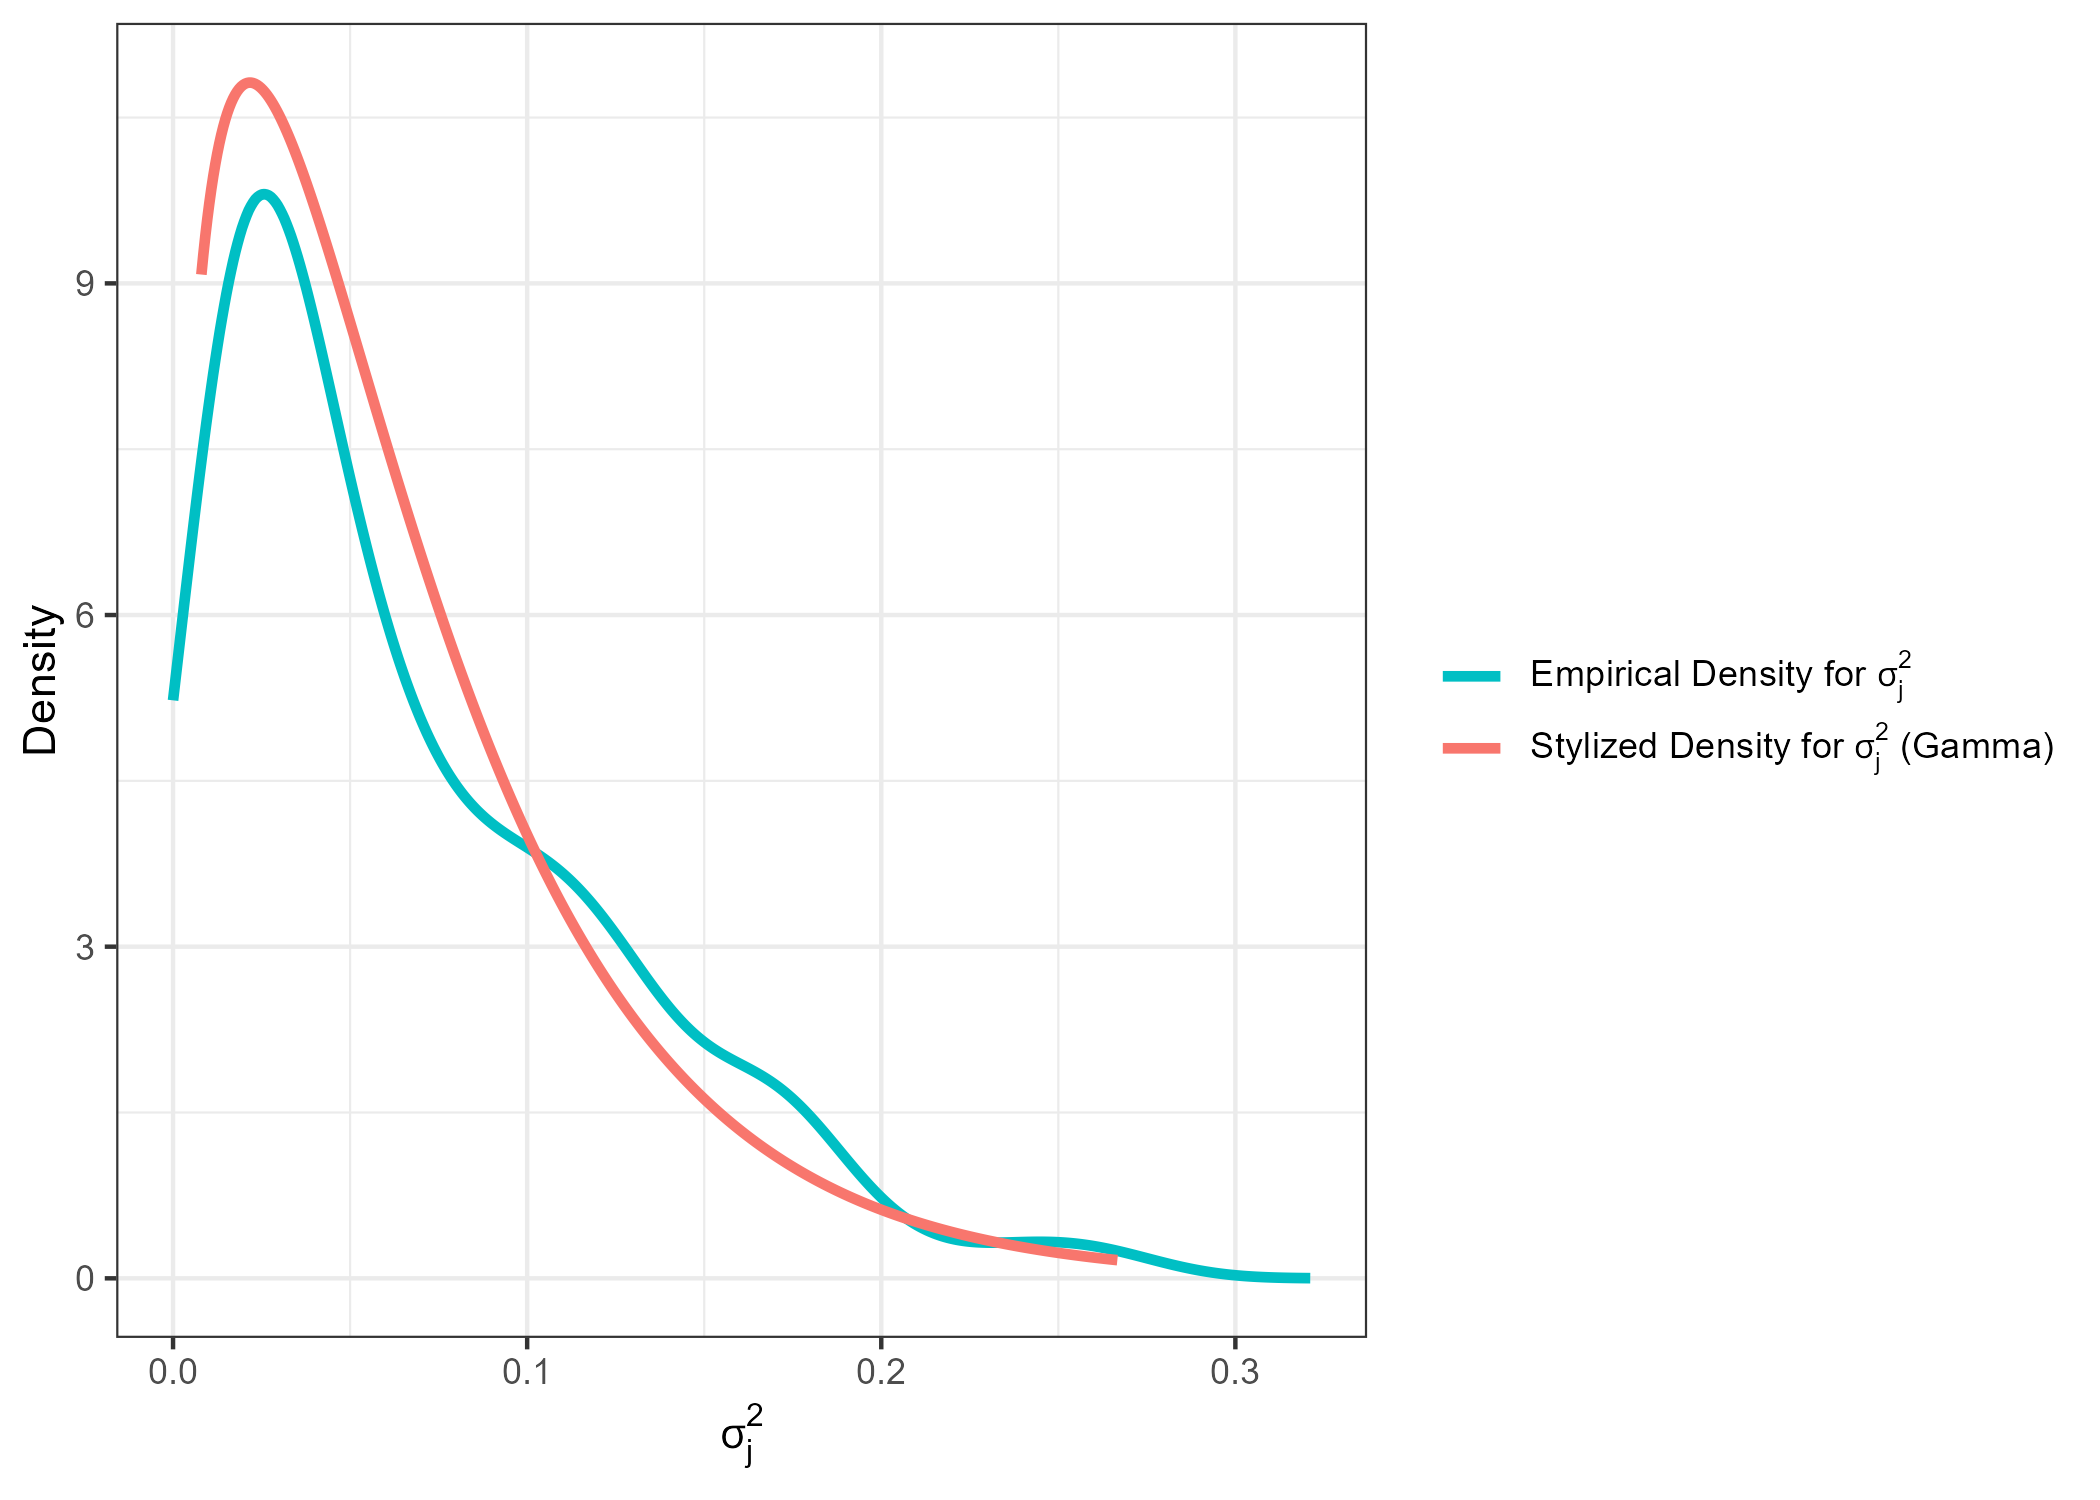
\includegraphics[width=\linewidth]{chapters/plots/densitysigma_j_sq.png}
    \caption{Density plots of $\sigma_j^2$ from Empirical vs Stylized Sampling Methods. \label{fig:densitysigma_sq}}
    \vspace{-5pt}
\end{figure}

\begin{figure}[H]
    \centering
    \vspace{-5pt}
    \includegraphics[width=\linewidth]{chapters/plots/pmfkj.png}
    \caption{PMF Plots of $k_j$ from Empirical vs Stylized Sampling Methods. \label{fig:pmfkj}}
    \vspace{-5pt}
\end{figure}

For the third method of obtaining $k_j$ and $\sigma_j^2$, the balanced assumption method, I estimate power assuming perfect balance where all the studies had the arithmetic means for $\sigma_j^2$ and $k_j$ of the empirical dataset from data generation, \textcite{WilliamsRyan2022HiMI}. This is the exact same way that the $\mu_c$ values are generated, so the approximation will return whatever the power neighborhood level, $P$,  is for that condition. Under this sampling method, we can see how different the true simulated power is from the power neighborhood value in that condition. 

\section{Simulation Design Conditions}\label{sec:simulationdesgin}

In this section, I detail the simulation design conditions. The factors that I examined included: (1) the number of categories ($C$), (2) the total number of studies ($J$), (3) the balance of the number of studies across categories (balanced $j_c$ vs. imbalanced $j_C$), (4) pattern type ($f_c$), (5) between-study heterogeneity ($\tau$), (6) within-study heterogeneity ($\omega$), (7) sampling correlation ($\rho$), and (8) power neighborhood ($P$). Table \ref{tab:experimentalconditions} summarizes the design conditions. In the following sections, I provide more details on each of the factors examined. 

% To validate the approximation, we will find the multiplier needed to give a power level. Given the rest of the meta-analytic data characteristics and the primary study characteristics, if you want to obtain a power level of $40\%$, how big does $\zeta$ need to be? 

\begin{table}[H]
\caption{Simulation Parameters}
     \label{tab:experimentalconditions}
    \centering
    \begin{tabular}{p{7cm}p{7cm}}
        \toprule
    Factor & Value \\ \midrule
       % Number of Categories ($C$) & 2, 3, 4 \\
       % Pattern Type ($f_c$) & AD or 50-50-Bal (8 patterns across $C$) \\

       Pattern Type ($f_c$)  & 2a, 3a, 3b, 3c, 4a, 4b, 4c, 4d \\
       Number of studies ($J$)  & 24, 36, 48, 60, 72  \\ 
       Between-study heterogeneity ($\tau$)  & 0.05, 0.20, 0.40 \\
       Within-study heterogeneity ($\omega$) & 0.05, 0.20 \\
       Sampling correlation ($\rho$) & .2, .5, .8 \\
       Power Neighborhood ($P$) & $5\%$ $20\%$, $40\%$, $60\%$, $80\%$, $90\%$ \\
       Balance of $j_c$ Across Categories & balanced $j_c$ vs imbalanced $j_c$ \\
        \bottomrule
    \end{tabular}
    \small
   % \caption{Caption}
\end{table}


\subsection{Pattern Type \texorpdfstring{($f_c$)}{ }} \label{sec: Pattern Type}
%and Number of Categories ($C$)


Table \ref{tab:patterns} and Section \ref{sec: patterns} detail the patterns of $\mu_c$ for each number of categories condition. For a given pattern, the first $\mu_c$ of each pattern was 0, and the rest of the $\mu_c$ is determined by the value of $\zeta$, which is found with the power neighborhood condition, study-level weights, $\tilde{w}_{jc}$, and a Type I error set to $\alpha = .05$. 

For the conditions, there are eight patterns across the values of $C$: one when $C = 2$, three when $C = 3$, and four when $C = 4$. They are denoted as:  2a, 3a, 3b, 3c, 4a, 4b, 4c, and 4d.  While there are many other potential values for the $\mu_c$, I choose these patterns because they offer a comprehensive set of $\mu_c$ values to evaluate when validating the power approximation. While the difference between each $\mu_c$ is a whole number times $\zeta$, it is possible to have any portion of $\zeta$ be the difference between categories; I decided only to add a multiple of $\zeta$ as a simplification. Additionally, the reason I set the first $\mu_c$ of each pattern to $0$ is that only the relative distance between $\mu_c$ matters for power. 

%\section{Meta-Meta Methods to Inform Experimental Conditions}
%Regarding the number of $C$ we evaluated, to better understand the characteristics of study-level category moderators, I coded additional information on study-level category moderators from the sample of studies from the meta-analytic dataset of \textcite{tipton2019}. \textcite{tipton2019} reviewed 64 meta-analyses to summarize the meta-analytic methods used in these studies. They coded variables related to the meta-analytic datasets and analyses, such as how many studies, samples, effect sizes, type of design, and the type of moderator analyses. For this dataset, for the meta-analyses that had study-level categorical moderators, I coded and summarized the number of categories.



%For this dataset, for the meta-analyses that had study-level categorical moderators, I coded and summarized the number of categories, number of studies per category, number of effect sizes per category, sample size per category, and magnitude of the overall effect size for each category. The results will inform the values used for my experimental conditions. After coding the additional information from these studies, I may adjust some of the proposed experimental conditions or the datasets used for data generation and validation. 

%Also could refer to these methodological articles for examples of what they did: Pustejovsky and Tipton 2015 2 - 6 Joshi et al. 2023 - for their conditions that use categorical moderators. 


\subsection{Number of Studies \texorpdfstring{($J$)}{ } and Balance of the Number of Studies across Categories (Balanced \texorpdfstring{$j_c$}{ } vs. imbalanced \texorpdfstring{$j_c$}{ })}

\subsubsection{Number of Studies, $J$}
I examined the following conditions for the number of studies per category: $J = 24, 36, 48, 60, 72$. Because the focus of this study is on the power of the Wald test of study-level categorical moderator, and $J$ should have a substantial impact, I decided on a large range of values for $J$ to better evaluate this factor. Additionally, I selected values that are multiples of 12, as they divide evenly into the values of $C$ in both levels of the balance, specifically the number of studies per category, $j_c$.  

I had also originally planned to look at $J=12$; however, before settling on the design conditions for the simulation study (see Table \ref{tab:experimentalconditions}), I first evaluated what each combination of parameters implies about the maximum $\mu_c$ values to see if any were unreasonably large. After generating the $\mu_c$ values, I graphed the maximum $\mu_c$ value of each $\bm{\beta}$.

Figure \ref{fig:max_mu} below displays all the generated maximum $\mu_c$ values of a $\bm{\beta}$ vector for the study, broken down by $f_c$, $\tau$, and $J$. There is some variation in the $\mu_c$ values beyond the factors in the Figure due to the $\rho$, $\omega$, and balance of the $j_c$ factors. In this study, the largest possible $\mu_c$ value is 1.43. Based on this exploration of the design conditions, I decided to remove $J=12$ condition because it resulted in a maximum $\mu_c$ value greater than 3 SD, which is not common in educational research \autocite{KraftMatthewA.2020IESo}.  The factors that seemed to have an impact on the magnitude of the $\mu_c$ values were $J$, $f_c$, $P$, the balance of the $j_c$, and $\tau$. The $\rho$ and $\omega$ had less of an impact on the magnitude of the max $\mu_c$ value. 

\begin{sidewaysfigure}
    \centering
    \vspace{-5pt}\includegraphics[width=\linewidth]{chapters/plots/max_mu.png}\caption{The max $\mu_c$ value by the pattern type ($f_c$), between-study heterogeneity ($\tau$), and the number of total studies ($J$). \label{fig:max_mu}}
    \vspace{-5pt}
\end{sidewaysfigure}


\subsubsection{Balanced $j_c$ vs. Imbalanced $j_c$ across $C$} 

For the balance of the $j_c$ condition, I looked at how the number of studies is distributed across the categories through two conditions: 1) balanced $j_c$ and 2) imbalanced $j_c$. The details of this condition are in Section \ref{sec: detailsbal}

The interaction between the distribution of the $\mu_c$ values in the $\bm{\beta}$ vector and the balance of the number of studies across the categories impacts power. I imposed various patterns of the $\mu_c$ intercepts for each of the categories (see Table \ref{tab:patterns}). Each pattern started with a known value of $\mu_1 = 0$, while at least one category had a $\mu_c$ that is greater than 0. By having the category with the largest $\mu_c$ value have the largest number of studies, then there should be more power for the Wald test of multiple categories. Since I aim to validate the approximation, I decided to make this simplification. While this is not exhaustive for the distribution of balance across a study-level categorical covariate, this setup demonstrates how extreme imbalances in the number of studies across categories and their interaction with the value of the $\beta$ slope impact power. 

The smallest number of studies per category, $j_c$, is $j_c = 4$ when there are imbalance $j_c$, $J = 24$, and the number of categories $C = 4$. The largest number of $j_c$ per category is when 54 studies are in one category, when $J= 72$, there are imbalanced $j_c$, and $C=2$. The extreme range of meta-analyses included in the simulated datasets is necessary to understand how the number of studies factor and the balance of the $j_c$ factor impact the power of a test for a categorical moderator. 

%While a categorical moderator only having $4$ studies is quite small, I have encountered categorical moderators that have that many studies within one category in practice.  


\subsection{Between-study Heterogeneity \texorpdfstring{($\tau$)}{ }, Within-study Heterogeneity \texorpdfstring{($\omega$)}{ }, and Sampling Correlation \texorpdfstring{($\rho$)}{ }}
For the values of between-study heterogeneity ($\tau$), within-study heterogeneity ($\omega$), and sampling correlation ($\rho$), I decided to follow the values used by \textcite{vembye2023}. For the between-study heterogeneity, the authors used $\tau = 0.05$, $0.2$, and $0.4$ to represent a small, medium, or large  $\tau$ value. They chose those values to match those observed across broad literature in social science meta-analyses \autocite{LindenAudreyHelen2021HoRR}. For the within-study heterogeneity, they used $\omega = 0.0$, $0.05$, $0.1$ and $0.20$ to represent no, small, medium, and large $\omega$ values, and that $\omega$ is typically smaller than $\tau$. For the sample correlation values, they evaluated $\rho = 0$ , $.2$, $.5$, $.8$, to represent no, small, moderate, and large $\rho$ values. I looked at the same conditions as well across the parameters, except I decided not to include  $\omega = 0$ and $\rho = 0$ conditions since I aim to validate the power approximation derived for the CHE model on data generated from CHE, while \textcite{vembye2023} also evaluated approximations for the CE and MLMA model for data generated from the CHE model. For my purposes, I chose not to look at special cases of the CHE model where there is no within-study variance or no correlation among effect sizes. To reduce the number of conditions and cut down on computational time, I chose not to include $\omega=0.1$. 

\subsection{Power Neighborhood}
For the power neighborhood levels, I decided to cover a large range of values: $5\%$, $20\%$, $40\%$, $60\%$, $80\%$, and $90\%$. The power level of $5\%$ is the Type I error rate because I set an $\alpha = .05$ for the nominal Type I error rate for the entire study. When the power neighborhood value equals the true Type I error rate, NCP was equal to 0, and I assessed the Type I error rate of the test. I decided to do a broad range for the rest of the power levels since I am trying to find NCP and, therefore, $\mu_c$ values from the power levels in combination with the other design factors.

%this is an artifice of this simulation to make sure we cover a range of conditions with respect to power. 


\subsection{Number of Conditions}

There are $8$ patterns across all the values of $C$, so I looked at those in combination. For this simulation study, there are $8$ values for $f_c$, $5$ values for $J$, $3$ values for $\tau$, $2$ values for $\omega$, $3$ values for $\rho$, $6$ values for $P$, and $2$ values for balance of $j_c$, resulting in $8640$ conditions.  


\subsection{Performance Criteria}
For this analysis, the primary performance criterion of interest is the discrepancy between the approximated power estimates and the true simulated power estimates found by the rejection rate for the cluster-robust Wald test using a CHE working model. The discrepancy is measured as the average of the approximated power estimates minus the rejection rates for each condition. Additionally, I am also interested in the nominal error rate of the cluster-robust Wald test when using a CHE working model, which is found when $ P=.05$. Below, I detail how I calculated the rejection rate for the simulated data, the MCSE of the rejection rate, the MCSE for the approximation estimates, and the MCSE for the discrepancy between the power estimates and the true power estimates. 

For the power estimates of the approximation results, $T$, with $K$ number of replications, the MCSE is:

\begin{equation}
    MCSE_{approx} = \sqrt{\frac{S^2_T}{K}}
\end{equation}
where $S_T^2$ is the sample variance, $S_T^2 = \frac{1}{K-1}\sum_{k=1}^K(T_k - \overline{T})^2$. 

I generated 150 power estimates using the approximation for each condition. I came up with 150 power estimates per condition by running some tests within one condition and calculating the MCSE. From these tests, I determined that I needed about 150 power estimates per condition to have MCSE values $\leq 0.01$. Then, I averaged the power estimates up to the condition level, resulting in $8640$ average power estimates.

For the simulated data, I calculated the rejection rate for the cluster-robust Wald test, which is the proportion of replications where a test returned a p-value less than the criterion $\alpha$-level: $\rho_{\alpha} = Pr(p_r < \alpha)$, where $R$ is the number of simulation iterations, $p_r$ is the p-value from replication $r$, $r = 1, \cdots, R$. The rejection rate is estimated as:
\begin{equation}
    r_{\alpha} = \frac{1}{R} \sum_{r=1}^R I(p_r < \alpha).
\end{equation}
The corresponding Monte Carlo standard error for the rejection rate estimate is (Morris et al., 2019):
\begin{equation}
    MCSE_{r_{\alpha}} = \sqrt{r_{\alpha}(1-r_{\alpha})/R}.
\end{equation}
I used $\alpha = .05$ for the rejection rate across all conditions. I compared the empirical rejection rate to the approximation results in each condition.

I generated 2,500 replications for each combination of conditions. By running 2,500 replications, the $MCSE < 0.01$ for every condition since with $r_{\alpha} = 0.5$, then $\sqrt{\frac{0.5(1-0.5)}{2500}} = 0.01$ (Please note, across all values of $r_{\alpha}$,  $ MCSE_{r_{\alpha}}$ is highest when $r_{\alpha} = 0.5$ ). 


Finally, because the approximated power and simulated power are independent, the MCSE of the discrepancy between the approximated power result and the true (simulated) power result is the following:

\begin{equation}
    \sqrt{MCSE_{r_{\alpha}}^2 + MCSE_{approx}^2}.
\end{equation}


\subsection{Analysis of Deviance for Power Discrepancies} \label{sec: analysis of deviance}

Following the methods of \textcite{vembye2023}, I ran a generalized linear model (GLM) on the power discrepancies for the empirical sampling method. I first transformed the approximation power results from probabilities to quantiles to be used in the "probit" link function (the cumulative standard normal distribution function), since this function converts probabilities to z-scores. Also, since the data is binomial (probability of rejection), the weights are set to the number of trials, which in this case is the number of iterations.  

Then, the transformed approximation power results are included in the formula as an offset term. Essentially, the model subtracts the offset z-score from the observed outcome z-score and then fits the linear predictors to that difference by including the offset (residual z-score).

In addition to this model, I also ran a GLM model on the rejection rates when $P=.05$ to test the nominal error. This model also used a "probit" link function, but did not include the offset term for the approximation power estimates, so the outcome was only the probability of rejection. 

Both models include the main effect for each factor and all the two-way interactions between factors. The only difference is that the model for the nominal error did not include the power neighborhood factor, $P$.  

I summarized the influence of each factor using an analysis of deviance, which I used to determine which factors to focus on when constructing the figures. I reported the deviance, which is the reduction in twice the log-likelihood for each term, where a higher deviance means more variation is explained in the outcome by that term. I did not assess the magnitude of each deviance, but I ranked all the deviances from largest to smallest and looked at the top 10 factors to get an idea of which factors were the most salient. 


\subsection{Details on Reproducibility}

All analyses were run on the University of Texas's Stampede3 supercomputer provided by the Texas Advanced Computing Center (TACC) (Skylake Compute Nodes; \url{https://docs.tacc.utexas.edu/hpc/stampede3/}). The code for this study can be found on \url{https://github.com/bethanyhamilton/PowerMeta_StudyCatMod}. Furthermore, for total replicability, I created Docker containers for the study. The Docker container allows you to completely control variables that may impact the results, like R or package versions, script versions, or even operating system differences in C-level linear algebra libraries. The simulation study is located here: \url{https://hub.docker.com/r/bethanyhamilton/powstudcatmod/tags} (version: v0), and the approximation study is located here: \url{https://hub.docker.com/r/bethanyhamilton/powstudcatmod_approx/tags} (version: v0). For this study, I used R \autocite[version 4.4.2;][]{R} with Linux kernel (version 5.15.153.1-microsoft-standard-WSL2). Linear algebra computations used LAPACK \autocite[version 3.12.0;][]{lapack99}. For the approximation study, I used the following R packages:
\texttt{mvtnorm}  \autocite[version 1.3-3;][]{mvtnorm}, \texttt{stringr}  \autocite[version 1.5.1;][]{stringr}, \texttt{purrr} \autocite[version 1.0.41;][]{purrr}, \texttt{dplyr} \autocite[version 1.1.4;][]{dplyr}, and \texttt{tidyr} \autocite[version 1.3.1;][]{tidyr}. In addition to these packages, for the simulation study, I also used \texttt{clubSandwich} \autocite[version 0.5.11;][]{pustejovsky2024a}  and \texttt{metafor} \autocite[version 4.8-0;][]{viechtbauer2010a}.


%\section{Implications} 
%summarize the expected contribution

%The results of this study will validate the power approximation for the tests of study-level category moderators in meta-regression of dependent effects. The results of my study can be directly applicable to applied meta-analysts who wish to conduct an a priori power analysis for their prospective meta-analytic study. Furthermore, this study will give more guidance on the performance and limitations the CHE+RVE model when it comes to the true power of the tests of study-level category moderators. 
%possible limitations ** 
%-these results can also be applied to Fisher-Z transformed correlation effect sizes. Still, the results will not translate to other effect size types like odds ratio without further assumptions \autocite{vembye2023}.

%Mention that we will not do pairwise comparisons. We have not yet done that --so I  need to find the joint distribution of the test statistics. 